% answers.tex —— 2001 年·全国新课程卷·理科 · 参考答案与详细解析片段
% 由 tools/generate_projects.py 依来源总账自 2001/2001_数学真题_全国新课程理_试题.md + 2001/2001_数学真题_全国新课程理_解析正文.md + 2001/2001_数学真题_全国新课程理_答案要点.md 生成，勿手改（改源 MD 后重跑）


\begin{gktip}
固定源 PDF 第 1–3 页为题面，第 4–8 页附有参考答案与评分标准。以下解析以第 1–3 页题面为对象独立复算；第 11、12、18、20（甲）、20（乙）、21 题的图形在 LaTeX 工程中以 TikZ/PGFPlots 矢量源重绘。
\end{gktip}

\gkpart{一、选择题}

\begin{answer}
\gksolhead{1}{}

\textbf{题目}：

函数 $y=3\sin\left(\dfrac{x}{2}+\dfrac\pi3\right)$ 的周期、振幅依次是\mbox{（　　）}

（A）$4\pi,\ 3$　　（B）$4\pi,\ -3$　　（C）$\pi,\ 3$　　（D）$\pi,\ -3$

\Needspace{4\baselineskip}
\textbf{解析}

\Needspace{5\baselineskip}
函数 $y=3\sin\left(\dfrac{x}{2}+\dfrac\pi3\right)$ 中，角变量的系数为 $\dfrac12$，所以周期为

\nopagebreak[4]
\[
T=\frac{2\pi}{1/2}=4\pi.
\]

振幅为 $|3|=3$，选 A。

\gkanswer{答案：A}

\end{answer}
\begin{answer}
\gksolhead{2}{}

\textbf{题目}：

若 $S_n$ 是数列 $\{a_n\}$ 的前 $n$ 项和，且 $S_n=n^2$，则 $\{a_n\}$ 是\mbox{（　　）}

（A）等比数列，但不是等差数列　　（B）等差数列，但不是等比数列

（C）等差数列，而且也是等比数列　　（D）既非等比数列又非等差数列

\Needspace{4\baselineskip}
\textbf{解析}

\Needspace{5\baselineskip}
由 $S_n=n^2$，有

\nopagebreak[4]
\[
a_1=S_1=1,\qquad
a_n=S_n-S_{n-1}=n^2-(n-1)^2=2n-1\quad(n\ge2).
\]

所以 $\{a_n\}$ 为首项 $1$、公差 $2$ 的等差数列。其相邻项之比不恒定，故不是等比数列，选 B。

\gkanswer{答案：B}

\end{answer}
\begin{answer}
\gksolhead{3}{}

\textbf{题目}：

过点 $A(1,-1)$、$B(-1,1)$ 且圆心在直线 $x+y-2=0$ 上的圆的方程是\mbox{（　　）}

（A）$(x-3)^2+(y+1)^2=4$　　（B）$(x+3)^2+(y-1)^2=4$

（C）$(x-1)^2+(y-1)^2=4$　　（D）$(x+1)^2+(y+1)^2=4$

\Needspace{4\baselineskip}
\textbf{解析}

\Needspace{5\baselineskip}
设圆锥轴截面为边长 $\ell$ 的等边三角形。由面积条件

\nopagebreak[4]
\[
\frac{\sqrt3}{4}\ell^2=\sqrt3,\qquad \ell=2.
\]

\Needspace{5\baselineskip}
轴截面的底边是圆锥底面直径，所以底面半径 $r=1$；轴截面的两腰是母线，母线长 $l=2$。圆锥全面积为

\nopagebreak[4]
\[
S_{\text{\text{全}}}=\pi r l+\pi r^2=2\pi+\pi=3\pi.
\]

选 C。

\gkanswer{答案：C}

\end{answer}
\begin{answer}
\gksolhead{4}{}

\textbf{题目}：

若定义在区间 $(-1,0)$ 内的函数 $f(x)=\log_{2a}(x+1)$ 满足 $f(x)>0$，则 $a$ 的取值范围是\mbox{（　　）}

（A）$\left(0,\dfrac12\right)$　　（B）$\left(0,\dfrac12\right]$　　（C）$\left(\dfrac12,+\infty\right)$　　（D）$(0,+\infty)$

\Needspace{4\baselineskip}
\textbf{解析}

\Needspace{5\baselineskip}
当 $x\in(-1,0)$ 时，$0<x+1<1$。要使 $\log_{2a}(x+1)>0$ 对区间内任意 $x$ 成立，底数必须满足

\nopagebreak[4]
\[
0<2a<1,
\]

即 $0<a<\dfrac12$。选 A。

\gkanswer{答案：A}

\end{answer}
\begin{answer}
\gksolhead{5}{}

\textbf{题目}：

若向量 $\boldsymbol a=(1,1)$，$\boldsymbol b=(1,-1)$，$\boldsymbol c=(-1,2)$，则 $\boldsymbol c=$\mbox{（　　）}

（A）$-\dfrac12\boldsymbol a+\dfrac32\boldsymbol b$　　（B）$\dfrac12\boldsymbol a-\dfrac32\boldsymbol b$

（C）$\dfrac32\boldsymbol a-\dfrac12\boldsymbol b$　　（D）$-\dfrac32\boldsymbol a+\dfrac12\boldsymbol b$

\Needspace{4\baselineskip}
\textbf{解析}

\Needspace{5\baselineskip}
设 $\boldsymbol c=u\boldsymbol a+v\boldsymbol b$，则

\nopagebreak[4]
\[
(u+v,u-v)=(-1,2).
\]

\Needspace{5\baselineskip}
解得 $u=\dfrac12$、$v=-\dfrac32$，所以

\nopagebreak[4]
\[
\boldsymbol c=\frac12\boldsymbol a-\frac32\boldsymbol b.
\]

选 B。

\gkanswer{答案：B}

\end{answer}
\begin{answer}
\gksolhead{6}{}

\textbf{题目}：

设 $A$、$B$ 是 $x$ 轴上的两点，点 $P$ 的横坐标为 $2$ 且 $|PA|=|PB|$。若直线 $PA$ 的方程为 $x-y+1=0$，则直线 $PB$ 的方程是\mbox{（　　）}

（A）$x+y-5=0$　　（B）$2x-y-1=0$　　（C）$2y-x-4=0$　　（D）$2x+y-7=0$

\Needspace{4\baselineskip}
\textbf{解析}

\Needspace{5\baselineskip}
直线 $PA$ 与 $x$ 轴交于

\nopagebreak[4]
\[
y=0,\quad x+1=0,
\]

\Needspace{5\baselineskip}
所以 $A=(-1,0)$。点 $P$ 的横坐标为 $2$，代入 $x-y+1=0$ 得 $P=(2,3)$。因 $|PA|=|PB|$ 且 $A,B$ 在 $x$ 轴上，$P$ 是线段 $AB$ 的垂直平分线上的点；由 $P$ 的横坐标为 $2$，得 $B=(5,0)$。直线 $PB$ 的方程为

\nopagebreak[4]
\[
x+y-5=0.
\]

选 A。

\gkanswer{答案：A}

\end{answer}
\begin{answer}
\gksolhead{7}{}

\textbf{题目}：

若 $0<\alpha<\beta<\dfrac\pi4$，$\sin\alpha+\cos\alpha=a$，$\sin\beta+\cos\beta=b$，则\mbox{（　　）}

（A）$a<b$　　（B）$a>b$　　（C）$ab<1$　　（D）$ab>2$

\Needspace{4\baselineskip}
\textbf{解析}

\Needspace{5\baselineskip}
令 $h(t)=\sin t+\cos t$。在 $(0,\pi/4)$ 内，

\nopagebreak[4]
\[
h'(t)=\cos t-\sin t>0.
\]

由于 $0<\alpha<\beta<\pi/4$，有 $a=h(\alpha)<h(\beta)=b$，选 A。

\gkanswer{答案：A}

\end{answer}
\begin{answer}
\gksolhead{8}{}

\textbf{题目}：

函数 $y=1+3x-x^3$ 有\mbox{（　　）}

（A）极小值 $-1$，极大值 $1$　　（B）极小值 $-2$，极大值 $3$

（C）极小值 $-2$，极大值 $2$　　（D）极小值 $-1$，极大值 $3$

\Needspace{4\baselineskip}
\textbf{解析}

\Needspace{5\baselineskip}
令 $f(x)=1+3x-x^3$，则

\nopagebreak[4]
\[
f'(x)=3-3x^2=3(1-x)(1+x).
\]

\Needspace{5\baselineskip}
因此 $f$ 在 $(-1,1)$ 上递增，在 $(-\infty,-1)$ 和 $(1,+\infty)$ 上递减。故极小值为

\nopagebreak[4]
\[
f(-1)=1-3+1=-1,
\]

\Needspace{5\baselineskip}
极大值为

\nopagebreak[4]
\[
f(1)=1+3-1=3.
\]

选 D。

\gkanswer{答案：D}

\end{answer}
\begin{answer}
\gksolhead{9}{}

\textbf{题目}：

某赛季足球比赛的计分规则是：胜一场，得 $3$ 分；平一场，得 $1$ 分；负一场，得 $0$ 分。一球队打完 $15$ 场，积 $33$ 分。若不考虑顺序，该队胜、负、平的情况共有\mbox{（　　）}

（A）$3$ 种　　（B）$4$ 种　　（C）$5$ 种　　（D）$6$ 种

\Needspace{4\baselineskip}
\textbf{解析}

\Needspace{5\baselineskip}
设胜、平、负的场数分别为 $w,d,l$，则

\nopagebreak[4]
\[
w+d+l=15,\qquad 3w+d=33.
\]

由此 $d=33-3w$、$l=2w-18$。非负整数条件给出 $9\le w\le11$，所以 $w$ 可取 $9,10,11$，共有 $3$ 种，选 A。

\gkanswer{答案：A}

\end{answer}
\begin{answer}
\gksolhead{10}{}

\textbf{题目}：

设坐标原点为 $O$，抛物线 $y^2=2x$ 与过焦点的直线交于 $A$、$B$ 两点，则 $\overrightarrow{OA}\cdot\overrightarrow{OB}=$\mbox{（　　）}

（A）$\dfrac34$　　（B）$-\dfrac34$　　（C）$3$　　（D）$-3$

\Needspace{4\baselineskip}
\textbf{解析}

\Needspace{5\baselineskip}
将抛物线 $y^2=2x$ 写成标准形式 $y^2=4ax$，得 $a=\dfrac12$。其参数方程为

\nopagebreak[4]
\[
P(t)=\left(\frac{t^2}{2},t\right),
\]

\Needspace{5\baselineskip}
焦点为 $F=(1/2,0)$。设 $A=P(t_1)$、$B=P(t_2)$，过这两点的弦方程为

\nopagebreak[4]
\[
2x-(t_1+t_2)y+t_1t_2=0.
\]

\Needspace{5\baselineskip}
代入焦点 $F$，得 $1+t_1t_2=0$，即 $t_1t_2=-1$。因此

\nopagebreak[4]
\[
\overrightarrow{OA}\cdot\overrightarrow{OB}
=\frac{t_1^2t_2^2}{4}+t_1t_2
=\frac14-1=-\frac34.
\]

选 B。

\gkanswer{答案：B}

\end{answer}
\begin{answer}
\gksolhead{11}{}

\textbf{题目}：

一间民房的屋顶有如图三种不同的盖法：① 单向倾斜；② 双向倾斜；③ 四向倾斜。记三种盖法屋顶面积分别为 $P_1$、$P_2$、$P_3$。若屋顶斜面与水平面所成的角都是 $\alpha$，则\mbox{（　　）}
\nopagebreak[4]
\begin{center}% 2001 年全国新课程卷理科第 11 题：三种屋顶盖法
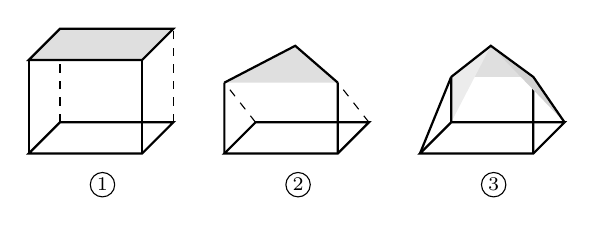
\begin{tikzpicture}[>=stealth, scale=0.72]
  \begin{scope}
    \coordinate (A) at (0,0);
    \coordinate (B) at (2.0,0);
    \coordinate (C) at (2.55,0.55);
    \coordinate (D) at (0.55,0.55);
    \coordinate (A1) at (0,1.65);
    \coordinate (B1) at (2.0,1.65);
    \coordinate (C1) at (2.55,2.2);
    \coordinate (D1) at (0.55,2.2);
    \draw[thick] (A)--(B)--(C)--(D)--cycle;
    \draw[thick] (A)--(A1) (B)--(B1);
    \draw[dashed] (C)--(C1) (D)--(D1);
    \fill[gray!25] (A1)--(B1)--(C1)--(D1)--cycle;
    \draw[thick] (A1)--(B1)--(C1)--(D1)--cycle;
    \node[circle,draw,inner sep=1pt] at (1.3,-0.55) {\scriptsize 1};
  \end{scope}
  \begin{scope}[xshift=3.45cm]
    \coordinate (A) at (0,0);
    \coordinate (B) at (2.0,0);
    \coordinate (C) at (2.55,0.55);
    \coordinate (D) at (0.55,0.55);
    \coordinate (M) at (1.25,1.9);
    \draw[thick] (A)--(B)--(C)--(D)--cycle;
    \draw[thick] (A)--(0,1.25) (B)--(2,1.25);
    \draw[dashed] (C)--(2,1.25) (D)--(0,1.25);
    \fill[gray!25] (0,1.25)--(M)--(2,1.25)--cycle;
    \draw[thick] (0,1.25)--(M)--(2,1.25);
    \node[circle,draw,inner sep=1pt] at (1.3,-0.55) {\scriptsize 2};
  \end{scope}
  \begin{scope}[xshift=6.9cm]
    \coordinate (A) at (0,0);
    \coordinate (B) at (2.0,0);
    \coordinate (C) at (2.55,0.55);
    \coordinate (D) at (0.55,0.55);
    \coordinate (M) at (1.25,1.9);
    \coordinate (L) at (0.55,1.35);
    \coordinate (R) at (2.0,1.35);
    \draw[thick] (A)--(B)--(C)--(D)--cycle;
    \draw[thick] (A)--(L) (B)--(R);
    \draw[dashed] (C)--(R) (D)--(L);
    \fill[gray!25] (L)--(M)--(R)--cycle;
    \fill[gray!15] (D)--(L)--(M)--cycle;
    \fill[gray!35] (M)--(R)--(C)--cycle;
    \draw[thick] (L)--(M)--(R) (D)--(L) (R)--(C);
    \node[circle,draw,inner sep=1pt] at (1.3,-0.55) {\scriptsize 3};
  \end{scope}
\end{tikzpicture}
\end{center}
\nopagebreak[4]
（A）$P_3>P_2>P_1$　　（B）$P_3>P_2=P_1$　　（C）$P_3=P_2>P_1$　　（D）$P_3=P_2=P_1$

\Needspace{4\baselineskip}
\textbf{解析}

\Needspace{5\baselineskip}
把每个屋顶斜面正投影到水平面。由于每个斜面与水平面的夹角都是 $\alpha$，斜面面积等于其水平投影面积除以 $\cos\alpha$。三种盖法覆盖的水平投影区域相同，因此

\nopagebreak[4]
\[
P_1=P_2=P_3.
\]

选 D。

\gkanswer{答案：D}

\end{answer}
\begin{answer}
\gksolhead{12}{}

\textbf{题目}：

如图，小圆圈表示网络的结点，结点之间的连线表示它们有网线相联。连线标注的数字表示该段网线单位时间内可以通过的最大信息量。现从结点 $A$ 向结点 $B$ 传递信息，信息可以分开沿不同的路线同时传递，则单位时间内传递的最大信息量是\mbox{（　　）}
\nopagebreak[4]
\begin{center}% 2001 年全国新课程卷理科第 12 题：信息网络
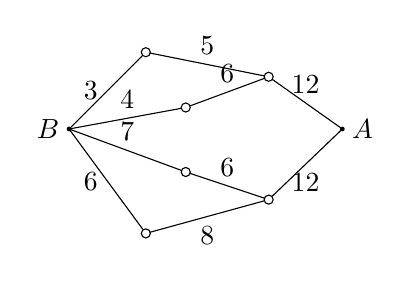
\begin{tikzpicture}[>=stealth, scale=0.78]
  \coordinate (B) at (0,0);
  \coordinate (U) at (1.25,1.25);
  \coordinate (V) at (3.25,0.85);
  \coordinate (M) at (1.9,0.35);
  \coordinate (N) at (1.9,-0.7);
  \coordinate (W) at (1.25,-1.7);
  \coordinate (Z) at (3.25,-1.15);
  \coordinate (A) at (4.45,0);

  \draw (B)--(U) node[midway, left] {3};
  \draw (U)--(V) node[midway, above] {5};
  \draw (B)--(M) node[midway, above] {4};
  \draw (M)--(V) node[midway, above] {6};
  \draw (B)--(N) node[midway, above] {7};
  \draw (N)--(Z) node[midway, above] {6};
  \draw (B)--(W) node[midway, left] {6};
  \draw (W)--(Z) node[midway, below] {8};
  \draw (V)--(A) node[midway, above] {12};
  \draw (Z)--(A) node[midway, below] {12};

  \foreach \point in {U,V,M,N,W,Z}
    \filldraw[fill=white] (\point) circle (2.1pt);
  \fill (B) circle (1.1pt) node[left] {$B$};
  \fill (A) circle (1.1pt) node[right] {$A$};
\end{tikzpicture}
\end{center}
\nopagebreak[4]
（A）$26$　　（B）$24$　　（C）$20$　　（D）$19$

\Needspace{4\baselineskip}
\textbf{解析}

虽然题面叙述传输方向为 $A$ 到 $B$，把所有边方向反向后容量问题等价；下面按图中从 $B$ 到 $A$ 计。将网络分成上、下两部分。上部从 $B$ 出发的两条边容量为 $3,4$，故上部最多传递 $7$；这 $7$ 单位可以分别沿容量为 $5,6$ 的边汇合后经容量为 $12$ 的边传到 $A$。

\Needspace{5\baselineskip}
下部汇合到右下结点的出口容量为 $12$，且可由 $B$ 到下部的容量 $7,6$ 及中间容量 $6,8$ 的边提供足够流量，所以可传递 $12$。因此总流量不超过

\nopagebreak[4]
\[
7+12=19.
\]

取上部流量 $3+4=7$，下部令两条支路各传 $6$，恰好得到总流量 $19$，故最大信息量为 $19$，选 D。

\gkanswer{答案：D}

\end{answer}
\gkpart{二、填空题}

\begin{answer}
\gksolhead{13}{}

\textbf{题目}：

若复数 $z=\sqrt2+\sqrt6\,i$，则 $\arg\dfrac1z$ 等于\gkblank{}。

\Needspace{4\baselineskip}
\textbf{解析}

\Needspace{5\baselineskip}
复数 $z=\sqrt2+\sqrt6\,i$ 位于第一象限，且

\nopagebreak[4]
\[
\tan\arg z=\frac{\sqrt6}{\sqrt2}=\sqrt3,
\]

\Needspace{5\baselineskip}
所以 $\arg z=\dfrac\pi3$。因此

\nopagebreak[4]
\[
\arg\frac1z=-\frac\pi3\equiv\frac{5\pi}{3}\pmod{2\pi}.
\]

\gkanswer{答案：$\dfrac{5\pi}{3}$}

\end{answer}
\begin{answer}
\gksolhead{14}{}

\textbf{题目}：

一个袋子里装有大小相同的 $3$ 个红球和 $2$ 个黄球。从中同时取出 $2$ 个，则其中含红球个数的数学期望是\gkblank{}。（用数字作答）

\Needspace{4\baselineskip}
\textbf{解析}

\Needspace{5\baselineskip}
设取出的两个球中红球个数为 $\xi$。由超几何分布，

\nopagebreak[4]
\[
P(\xi=0)=\frac{\binom20\binom32}{\binom52}=\frac1{10},\quad
P(\xi=1)=\frac{\binom21\binom31}{\binom52}=\frac6{10},\quad
P(\xi=2)=\frac{\binom22\binom30}{\binom52}=\frac3{10}.
\]

\Needspace{5\baselineskip}
所以

\nopagebreak[4]
\[
E(\xi)=0\cdot\frac1{10}+1\cdot\frac6{10}+2\cdot\frac3{10}
=\frac65=1.2.
\]

\gkanswer{答案：$1.2$}

\end{answer}
\begin{answer}
\gksolhead{15}{}

\textbf{题目}：

在空间中，①若四点不共面，则这四点中任何三点都不共线；②若两条直线没有公共点，则这两条直线是异面直线。以上两个命题中，逆命题为真命题的是\gkblank{}。（把符合要求的命题序号都填上）

\Needspace{4\baselineskip}
\textbf{解析}

命题①的逆命题是“若四点中任何三点都不共线，则四点不共面”。四个点在同一平面内且处于一般位置时，任何三点也可以不共线，因此该逆命题不一定成立。

命题②的逆命题是“若两条直线是异面直线，则两条直线没有公共点”。异面直线按定义不共面，也不相交，故没有公共点，该逆命题为真。

因此应填②。

\gkanswer{答案：②}

\end{answer}
\begin{answer}
\gksolhead{16}{}

\textbf{题目}：

设 $\{a_n\}$ 是公比为 $q$ 的等比数列，$S_n$ 是它的前 $n$ 项和。若 $\{S_n\}$ 是等差数列，则 $q=$\gkblank{}。

\Needspace{4\baselineskip}
\textbf{解析}

\Needspace{5\baselineskip}
因为 $S_{n+1}-S_n=a_{n+1}$，若 $\{S_n\}$ 为等差数列，则 $a_{n+1}$ 为常数。按等比数列的定义，公比 $q\ne0$ 且各项可作相邻项之比，所以 $a_2\ne0$；由 $a_2=a_3$ 得

\nopagebreak[4]
\[
a_2q=a_2,\qquad q=1.
\]

\gkanswer{答案：$1$}

\end{answer}
\gkpart{三、解答题}

\begin{answer}
\gksolhead{17}{}

\textbf{题目}：

\Needspace{5\baselineskip}
解关于 $x$ 的不等式

\nopagebreak[4]
\[
\frac{x-a}{x-a^2}<0\qquad(a\in\mathbb R).
\]

\Needspace{4\baselineskip}
\textbf{解析}

\Needspace{5\baselineskip}
不等式为

\nopagebreak[4]
\[
\frac{x-a}{x-a^2}<0,\qquad x\ne a^2.
\]

\Needspace{5\baselineskip}
当 $a<0$ 或 $a>1$ 时，$a<a^2$，分式在两个根之间为负，解集为

\nopagebreak[4]
\[
a<x<a^2.
\]

\Needspace{5\baselineskip}
当 $0<a<1$ 时，$a^2<a$，分式在两个根之间为负，解集为

\nopagebreak[4]
\[
a^2<x<a.
\]

\Needspace{5\baselineskip}
当 $a=0$ 或 $a=1$ 时，分子、分母分别恒等或相同，严格不等式没有解。因此综上：

\nopagebreak[4]
\[
\begin{cases}
a<x<a^2,&a<0\text{ \text{或} }a>1,\\
a^2<x<a,&0<a<1,\\
\varnothing,&a=0\text{ \text{或} }a=1.
\end{cases}
\]

\gkanswer{答案：当 $a<0$ 或 $a>1$ 时，$a<x<a^2$；当 $0<a<1$ 时，$a^2<x<a$；当 $a=0$ 或 $a=1$ 时无解。}

\end{answer}
\begin{answer}
\gksolhead{18}{}

\textbf{题目}：

如图，用 $A$、$B$、$C$ 三类不同的元件连接成两个系统 $N_1$、$N_2$。当元件 $A$、$B$、$C$ 都正常工作时，系统 $N_1$ 正常工作；当元件 $A$ 正常工作且元件 $B$、$C$ 至少有一个正常工作时，系统 $N_2$ 正常工作。已知元件 $A$、$B$、$C$ 正常工作的概率依次为 $0.80,0.90,0.90$。
\nopagebreak[4]
\begin{center}% 2001 年全国新课程卷理科第 18 题：两个元件系统
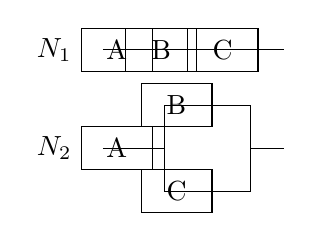
\begin{tikzpicture}[>=stealth, scale=0.78]
  \tikzset{component/.style={draw, rectangle, minimum width=0.9cm,
    minimum height=0.55cm, inner sep=1pt}}
  \node[left] at (0,1.45) {$N_1$};
  \draw (0.35,1.45)--(0.8,1.45)
    node[component, midway] {A}
    --(1.8,1.45)
    node[component, midway] {B}
    --(2.8,1.45)
    node[component, midway] {C}
    --(3.3,1.45);

  \node[left] at (0,-0.15) {$N_2$};
  \draw (0.35,-0.15)--(0.8,-0.15)
    node[component, midway] {A}
    --(1.35,-0.15);
  \draw (1.35,-0.15)--(1.35,0.55)--(1.75,0.55)
    node[component, midway] {B}
    --(2.75,0.55)--(2.75,-0.15);
  \draw (1.35,-0.15)--(1.35,-0.85)--(1.75,-0.85)
    node[component, midway] {C}
    --(2.75,-0.85)--(2.75,-0.15);
  \draw (2.75,-0.15)--(3.3,-0.15);
\end{tikzpicture}
\end{center}
\nopagebreak[4]
（1） 求系统 $N_1$ 正常工作的概率 $P_1$；

（2） 求系统 $N_2$ 正常工作的概率 $P_2$。

\Needspace{4\baselineskip}
\textbf{解析}

\Needspace{5\baselineskip}
由题设，三个元件正常工作的事件相互独立，且

\nopagebreak[4]
\[
P(A)=0.80,\qquad P(B)=0.90,\qquad P(C)=0.90.
\]

\gksubpart{(1)}

\Needspace{5\baselineskip}
系统 $N_1$ 正常工作当且仅当 $A,B,C$ 都正常，所以

\nopagebreak[4]
\[
P_1=P(A)P(B)P(C)
=0.80\times0.90\times0.90=0.648.
\]

\gksubpart{(2)}

\Needspace{5\baselineskip}
系统 $N_2$ 正常工作当且仅当 $A$ 正常且 $B,C$ 至少有一个正常。故

\nopagebreak[4]
\[
\begin{aligned}
P_2
&=P(A)\left[1-P(\overline B\cap\overline C)\right]\\
&=0.80\left[1-(1-0.90)(1-0.90)\right]\\
&=0.80\times0.99=0.792.
\end{aligned}
\]

\gkanswer{答案（1）：$P_1=0.648$。}

\gkanswer{答案（2）：$P_2=0.792$。}

\end{answer}
\begin{answer}
\gksolhead{19}{}

\textbf{题目}：

设 $a>0$，$f(x)=\dfrac{e^x}{a}+\dfrac{a}{e^x}$ 是 $\mathbb R$ 上的偶函数。

（1） 求 $a$ 的值；

（2） 证明 $f(x)$ 在 $(0,+\infty)$ 上是增函数。

\Needspace{4\baselineskip}
\textbf{解析}

\gksubpart{(1)}

\Needspace{5\baselineskip}
由 $f(x)$ 为偶函数，对任意 $x$ 有

\nopagebreak[4]
\[
\frac{e^{-x}}a+\frac{a}{e^{-x}}
=\frac{e^x}a+\frac{a}{e^x}.
\]

\Needspace{5\baselineskip}
整理得

\nopagebreak[4]
\[
\left(a-\frac1a\right)(e^x-e^{-x})=0.
\]

\Needspace{5\baselineskip}
取 $x=1$，因 $e-e^{-1}\ne0$，故 $a-\dfrac1a=0$。又 $a>0$，所以

\nopagebreak[4]
\[
a=1.
\]

\gksubpart{(2)}

\Needspace{5\baselineskip}
代入 $a=1$，得

\nopagebreak[4]
\[
f(x)=e^x+e^{-x}.
\]

\Needspace{5\baselineskip}
当 $x>0$ 时，

\nopagebreak[4]
\[
f'(x)=e^x-e^{-x}>0.
\]

所以 $f(x)$ 在 $(0,+\infty)$ 上是增函数。

\gkanswer{答案（1）：$a=1$。}

\gkanswer{答案（2）：$f(x)$ 在 $(0,+\infty)$ 上是增函数。}

\end{answer}
\begin{answer}
\gksolhead{20}{}

\textbf{题目}：

注意：考生在（20 甲）、（20 乙）两题中选一题作答，如果两题都答，只以（20 甲）计分。

【甲】如图，以正四棱锥 $V-ABCD$ 底面中心 $O$ 为坐标原点建立空间直角坐标系 $O-xyz$，其中 $Ox\parallel BC$，$Oy\parallel AB$。$E$ 为 $VC$ 中点，正四棱锥底面边长为 $2a$，高为 $h_0$。
\nopagebreak[4]
\begin{center}% 2001 年全国新课程卷理科第 20 题甲：正四棱锥坐标图
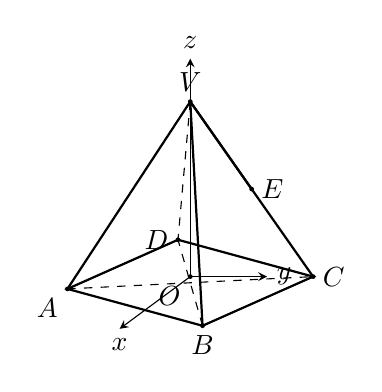
\begin{tikzpicture}[>=stealth, scale=0.78]
  \coordinate (A) at (-2.0,-0.4);
  \coordinate (B) at (0.2,-1.0);
  \coordinate (C) at (2.0,-0.2);
  \coordinate (D) at (-0.2,0.4);
  \coordinate (O) at (0, -0.2);
  \coordinate (V) at (0,2.65);
  \coordinate (E) at (1.0,1.225);

  \draw[thick] (A)--(B)--(C)--(D)--cycle;
  \draw[dashed] (A)--(C) (B)--(D);
  \draw[thick] (V)--(A) (V)--(B) (V)--(C);
  \draw[dashed] (V)--(D);
  \draw[thick] (V)--(E);
  \fill (A) circle (1.1pt) node[below left] {$A$};
  \fill (B) circle (1.1pt) node[below] {$B$};
  \fill (C) circle (1.1pt) node[right] {$C$};
  \fill (D) circle (1.1pt) node[left] {$D$};
  \fill (O) circle (1.1pt) node[below left] {$O$};
  \fill (V) circle (1.1pt) node[above] {$V$};
  \fill (E) circle (1.1pt) node[right] {$E$};
  \draw[->] (O)--(-1.15,-1.05) node[below] {$x$};
  \draw[->] (O)--(1.25,-0.2) node[right] {$y$};
  \draw[->] (O)--(0,3.35) node[above] {$z$};
\end{tikzpicture}
\end{center}
\nopagebreak[4]
（1） 求 $\cos\langle\overrightarrow{BE},\overrightarrow{DE}\rangle$；

（2） 记面 $BCV$ 为 $\alpha$，面 $DCV$ 为 $\beta$，若 $\angle BED$ 是二面角 $\alpha-VC-\beta$ 的平面角，求 $\angle BED$。

【乙】如图，在底面是直角梯形的四棱锥 $S-ABCD$ 中，$\angle ABC=90^\circ$，$SA\perp$ 面 $ABCD$，$SA=AB=BC=1$，$AD=\dfrac12$。
\nopagebreak[4]
\begin{center}% 2001 年全国新课程卷理科第 20 题乙：直角梯形底面的四棱锥
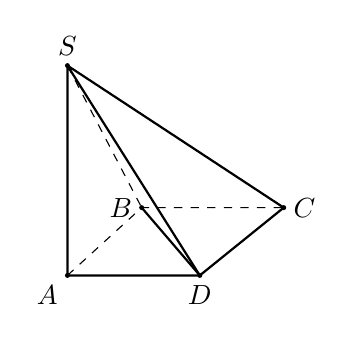
\begin{tikzpicture}[>=stealth, scale=0.82]
  \coordinate (A) at (0,0);
  \coordinate (B) at (1.15,1.05);
  \coordinate (C) at (3.35,1.05);
  \coordinate (D) at (2.05,0);
  \coordinate (S) at (0,3.25);

  \draw[thick] (S)--(A) (S)--(C) (S)--(D);
  \draw[dashed] (S)--(B);
  \draw[thick] (A)--(D)--(C);
  \draw[dashed] (A)--(B)--(C);
  \draw[thick] (B)--(D);

  \fill (S) circle (1.1pt) node[above] {$S$};
  \fill (A) circle (1.1pt) node[below left] {$A$};
  \fill (B) circle (1.1pt) node[left] {$B$};
  \fill (C) circle (1.1pt) node[right] {$C$};
  \fill (D) circle (1.1pt) node[below] {$D$};
\end{tikzpicture}
\end{center}
\nopagebreak[4]
（1） 求四棱锥 $S-ABCD$ 的体积；

（2） 求面 $SCD$ 与面 $SBA$ 所成的二面角的正切值。

\Needspace{4\baselineskip}
\textbf{解析}

\gksubpart{(1)}

\Needspace{5\baselineskip}
甲题中取坐标

\nopagebreak[4]
\[
B=(a,a,0),\quad C=(-a,a,0),\quad D=(-a,-a,0),\quad
V=(0,0,h_0).
\]

\Needspace{5\baselineskip}
由于 $E$ 是 $VC$ 的中点，

\nopagebreak[4]
\[
E=\left(-\frac a2,\frac a2,\frac{h_0}{2}\right).
\]

\Needspace{5\baselineskip}
因此

\nopagebreak[4]
\[
\overrightarrow{BE}=\left(-\frac{3a}{2},-\frac a2,\frac{h_0}{2}\right),
\qquad
\overrightarrow{DE}=\left(\frac a2,\frac{3a}{2},\frac{h_0}{2}\right).
\]

\Needspace{5\baselineskip}
于是

\nopagebreak[4]
\[
\overrightarrow{BE}\cdot\overrightarrow{DE}
=-\frac{3a^2}{2}+\frac{h_0^2}{4},
\]

\Needspace{5\baselineskip}
且

\nopagebreak[4]
\[
|\overrightarrow{BE}|=|\overrightarrow{DE}|
=\frac12\sqrt{10a^2+h_0^2}.
\]

\Needspace{5\baselineskip}
故

\nopagebreak[4]
\[
\cos\langle\overrightarrow{BE},\overrightarrow{DE}\rangle
=\frac{h_0^2-6a^2}{h_0^2+10a^2}.
\]

\Needspace{5\baselineskip}
乙题中使用与题面一致的坐标

\nopagebreak[4]
\[
B=(0,0,0),\quad C=(1,0,0),\quad A=(0,1,0),\quad
D=\left(\frac12,1,0\right),\quad S=(0,1,1).
\]

\Needspace{5\baselineskip}
底面直角梯形的面积为

\nopagebreak[4]
\[
S_{ABCD}=\frac{(AD+BC)\cdot AB}{2}
=\frac34,
\]

\Needspace{5\baselineskip}
所以四棱锥体积为

\nopagebreak[4]
\[
V=\frac13S_{ABCD}\cdot SA=\frac14.
\]

\gksubpart{(2)}

\Needspace{5\baselineskip}
甲题中，若 $\angle BED$ 是二面角 $\alpha-VC-\beta$ 的平面角，则

\nopagebreak[4]
\[
\overrightarrow{BE}\perp\overrightarrow{CV}.
\]

\Needspace{5\baselineskip}
而

\nopagebreak[4]
\[
\overrightarrow{CV}=(a,-a,h_0),
\]

\Needspace{5\baselineskip}
故

\nopagebreak[4]
\[
\overrightarrow{BE}\cdot\overrightarrow{CV}
=-\frac{3a^2}{2}+\frac{a^2}{2}+\frac{h_0^2}{2}=0,
\]

\Needspace{5\baselineskip}
从而 $h_0=\sqrt2a$。代回上式，

\nopagebreak[4]
\[
\cos\angle BED=-\frac13.
\]

\Needspace{5\baselineskip}
所以

\nopagebreak[4]
\[
\angle BED=\arccos\left(-\frac13\right)
=\pi-\arccos\frac13.
\]

\Needspace{5\baselineskip}
乙题中，平面 $SBA$ 的法向量可取

\nopagebreak[4]
\[
\boldsymbol n_1=(1,0,0).
\]

\Needspace{5\baselineskip}
又

\nopagebreak[4]
\[
\overrightarrow{SC}=(1,-1,-1),\qquad
\overrightarrow{SD}=\left(\frac12,0,-1\right),
\]

\Needspace{5\baselineskip}
故平面 $SCD$ 的法向量可取

\nopagebreak[4]
\[
\boldsymbol n_2=\overrightarrow{SC}\times\overrightarrow{SD}
=\left(1,\frac12,\frac12\right).
\]

\Needspace{5\baselineskip}
设两平面所成的锐二面角为 $\varphi$，则

\nopagebreak[4]
\[
\cos\varphi=\frac{|\boldsymbol n_1\cdot\boldsymbol n_2|}
{|\boldsymbol n_1|\,|\boldsymbol n_2|}
=\frac1{\sqrt6/2}=\sqrt{\frac23}.
\]

\Needspace{5\baselineskip}
于是

\nopagebreak[4]
\[
\tan\varphi=\sqrt{\frac1{\cos^2\varphi}-1}
=\sqrt{\frac32-1}=\frac{\sqrt2}{2}.
\]

\gkanswer{答案（1）：甲：$\dfrac{h_0^2-6a^2}{h_0^2+10a^2}$；乙：$\dfrac14$。}

\gkanswer{答案（2）：甲：$\pi-\arccos\dfrac13$；乙：$\dfrac{\sqrt2}{2}$。}

\end{answer}
\begin{answer}
\gksolhead{21}{}

\textbf{题目}：

某电厂冷却塔的外形是如图所示双曲线的一部分绕其中轴（即双曲线的虚轴）旋转所成的曲面，其中 $A,A'$ 是双曲线的顶点，$C,C'$ 是冷却塔上口直径的两个端点，$B,B'$ 是下底直径的两个端点，已知 $AA'=14\ \mathrm m$，$CC'=18\ \mathrm m$，$BB'=22\ \mathrm m$，塔高 $20\ \mathrm m$。

（1） 建立坐标系并写出该双曲线方程；

（2） 求冷却塔的容积（精确到 $10\ \mathrm m^3$，塔壁厚度不计，$\pi$ 取 $3.14$）。
\nopagebreak[4]
\begin{center}% 2001 年全国新课程卷理科第 21 题：冷却塔双曲线截面
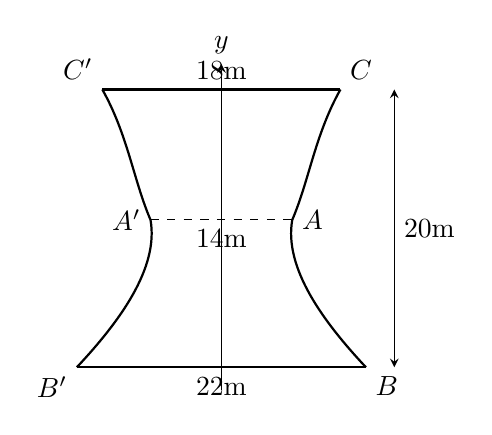
\begin{tikzpicture}[>=stealth, scale=0.72]
  \coordinate (TL) at (-2.1,2.45);
  \coordinate (TR) at (2.1,2.45);
  \coordinate (ML) at (-1.25,0.15);
  \coordinate (MR) at (1.25,0.15);
  \coordinate (BL) at (-2.55,-2.45);
  \coordinate (BR) at (2.55,-2.45);

  \draw[thick] (TL) .. controls (-1.65,1.65) and (-1.55,0.85) .. (ML)
    .. controls (-1.1,-0.7) and (-1.8,-1.65) .. (BL);
  \draw[thick] (TR) .. controls (1.65,1.65) and (1.55,0.85) .. (MR)
    .. controls (1.1,-0.7) and (1.8,-1.65) .. (BR);
  \draw[thick] (TL)--(TR) node[midway, above] {$18\mathrm{m}$};
  \draw[thick] (BL)--(BR) node[midway, below] {$22\mathrm{m}$};
  \draw[dashed] (ML)--(MR) node[midway, below] {$14\mathrm{m}$};
  \draw[<->] (3.05,-2.45)--(3.05,2.45) node[midway, right] {$20\mathrm{m}$};
  \draw[->] (0,-2.85)--(0,2.9) node[above] {$y$};
  \node[above left] at (TL) {$C'$};
  \node[above right] at (TR) {$C$};
  \node[left] at (ML) {$A'$};
  \node[right] at (MR) {$A$};
  \node[below left] at (BL) {$B'$};
  \node[below right] at (BR) {$B$};
\end{tikzpicture}
\end{center}
\nopagebreak[4]
\Needspace{4\baselineskip}
\textbf{解析}

\gksubpart{(1)}

\Needspace{5\baselineskip}
建立直角坐标系：取双曲线中心为原点 $O$，横轴为 $x$ 轴，竖直中轴为 $y$ 轴。设双曲线方程为

\nopagebreak[4]
\[
\frac{x^2}{a^2}-\frac{y^2}{b^2}=1.
\]

\Needspace{5\baselineskip}
由 $AA'=14$ 得 $a=7$。冷却塔上口、下底的半径分别为 $9$ m、$11$ m，且塔高为 $20$ m。令上口所在高度为 $y=8$，下底所在高度为 $y=-12$，则

\nopagebreak[4]
\[
C=(9,8),\qquad B=(11,-12).
\]

\Needspace{5\baselineskip}
代入双曲线方程，分别得到

\nopagebreak[4]
\[
\frac{9^2}{7^2}-\frac{8^2}{b^2}=1,\qquad
\frac{11^2}{7^2}-\frac{(-12)^2}{b^2}=1.
\]

\Needspace{5\baselineskip}
两式均给出 $b^2=98$，所以双曲线方程为

\nopagebreak[4]
\[
\frac{x^2}{49}-\frac{y^2}{98}=1.
\]

\gksubpart{(2)}

\Needspace{5\baselineskip}
由方程得旋转截面的半径平方为

\nopagebreak[4]
\[
x^2=\frac12y^2+49,\qquad -12\le y\le8.
\]

\Needspace{5\baselineskip}
绕 $y$ 轴旋转所得容积为

\nopagebreak[4]
\[
\begin{aligned}
V
&=\pi\int_{-12}^{8}x^2\,\mathrm dy\\
&=\pi\int_{-12}^{8}\left(\frac12y^2+49\right)\mathrm dy\\
&=\pi\left[\frac{y^3}{6}+49y\right]_{-12}^{8}\\
&=\frac{4060\pi}{3}.
\end{aligned}
\]

\Needspace{5\baselineskip}
取 $\pi=3.14$，得

\nopagebreak[4]
\[
V\approx4.2495\times10^3\ \mathrm m^3.
\]

精确到 $10\ \mathrm m^3$ 为 $4.25\times10^3\ \mathrm m^3$。

\gkanswer{答案（1）：双曲线方程为 $\dfrac{x^2}{49}-\dfrac{y^2}{98}=1$。}

\gkanswer{答案（2）：冷却塔容积约为 $4.25\times10^3\ \mathrm m^3$。}

\end{answer}
\begin{answer}
\gksolhead{22}{}

\textbf{题目}：

\Needspace{5\baselineskip}
设 $0<\theta<\dfrac\pi2$，曲线

\nopagebreak[4]
\[
x^2\sin\theta+y^2\cos\theta=1
\]

\Needspace{5\baselineskip}
和

\nopagebreak[4]
\[
x^2\cos\theta-y^2\sin\theta=1
\]

有 $4$ 个不同的交点。

（1） 求 $\theta$ 的取值范围；

（2） 证明这 $4$ 个交点共圆，并求圆半径的取值范围。

\Needspace{4\baselineskip}
\textbf{解析}

\gksubpart{(1)}

\Needspace{5\baselineskip}
设交点为 $(x,y)$。两曲线方程相加、相减可得

\nopagebreak[4]
\[
\begin{cases}
x^2=\sin\theta+\cos\theta,\\
y^2=\cos\theta-\sin\theta.
\end{cases}
\]

\Needspace{5\baselineskip}
在 $0<\theta<\pi/2$ 内，$\sin\theta+\cos\theta>0$ 恒成立。要有四个不同的交点，必须同时有 $x^2>0$、$y^2>0$，因此

\nopagebreak[4]
\[
\cos\theta-\sin\theta>0
\Longleftrightarrow 0<\theta<\frac\pi4.
\]

\gksubpart{(2)}

\Needspace{5\baselineskip}
由上面的交点坐标关系，

\nopagebreak[4]
\[
x^2+y^2
=\sin\theta+\cos\theta+\cos\theta-\sin\theta
=2\cos\theta.
\]

\Needspace{5\baselineskip}
所以四个交点都在以原点为圆心、半径

\nopagebreak[4]
\[
r=\sqrt{2\cos\theta}
\]

\Needspace{5\baselineskip}
的圆上。又 $0<\theta<\pi/4$，且 $\cos\theta$ 在该区间内递减，故

\nopagebreak[4]
\[
\sqrt[4]{2}<r<\sqrt2.
\]

\gkanswer{答案（1）：$0<\theta<\dfrac\pi4$。}

\gkanswer{答案（2）：圆半径 $r$ 的取值范围为 $\left(\sqrt[4]{2},\sqrt2\right)$。}

\end{answer}